In einem Abstand von circa 4,5 m vom Kollisionspunkt deckt das EMCal einen Azimuthalwinkelbereich von $\phi=107^{\circ}$ und einen Pseudorapidit\"atsbreich von $ |\eta| \leq 0\,7$ ab.
%Aufgrund von Detektormaterial und Tr\"agerstrukturen zwischen dem prim\"aren Vertex und dem EMCal k\"onnen Teilchen abgelenkt werden oder Photonen in ein Elektron-Positron-Paar konvertieren.
%Die Konvertierung von Photonen ist besonders zu beachten, da in dieser Analyse $\pi^{0}$, welche in zwei Photonen zerfallen, rekonstruiert werden.
Das EMCal besteht aus zw\"olf sogenannten Supermodulen, zehn normal gro{\ss}en und zwei kleinere.
Ein normal gro{\ss}es Supermodul besteht aus $24\cdot48$ Zellen, ein kleineres Supermodul aus $8\cdot48$ Zellen.
Insgesamt hat das EMCal also 12288 Zellen, die haupts\"achlich Photonen, Elektronen und Positronen detektieren und dabei die Energie dieser Teilchen messen.
%Ein normal gro{\ss}es Supermodul unterteilt sich in 24 sogenannte Streifenmodule, welche wiederum aus 12 Modulen zusammengesetzt sind.
%Jedes Modul beinhaltet 4 Zellen, womit das EMCal aus insgesamt 12288 Zellen besteht.
%Die Zellen sind f\"ur das Detektieren und Messen der Energie von haupts\"achlich Photonen, Elektronen und Positronen verantwortlich.
Eine einzelne Zelle besteht aus abwechselnd 77 Szintillatoren- und 76 Bleischichten.
In den Bleischichten entstehen sogenannten elektromagnetische Schauer, indem eintreffende Photonen durch Paarerzeugung in ein Elektron und ein Positron konvertieren, die wiederum durch Bremsstrahlung weitere Photonen abstrahlen.
Die Szintillatoren werden durch die Photonen angeregt und geben ein messbares Lichtsignal ab.
Alle Szintillatorschichten einer Zelle sind \"uber einen Lichtleiter mit einem Photomultiplier verbunden.
Der Photomultiplier wandelt das Lichtsignal in ein elektrisches Signal um, das proportional zur detektierten Energie der Zelle ist.
\newline
Jeder elektromagnetischer Schauer besitzt eine gewisse Ausdehnung, die \"uber den sogenannten Moli\`ere-Radius $R_{\text{M}}$ definiert ist.
Der Moli\`ere-Radius gibt den Radius passend zu einem Zylinder an, in dem 90\% der gesamten Energie eines Schauers vom Detektor gemessen wird.
F\"ur das EMCal betr\"agt der Moli\`ere-Radius $R_{\text{M}} = 3\,7$ cm, w\"ahrend die quadratischen Zellen eine Seitenl\"ange von 6 cm besitzen. 
Der Schauer eines einzelnen Teilchens erstreckt sich also \"uber mehrere Zellen.
Benachbarte Zellen werden durch einen Algorithmus zu sogenannten \textit{Clustern} zusammengefasst.
Algorithmen zur Rekonstruktion von \textit{Clustern} werden als \textit{Clusterizer} bezeichnet.
In der hier vorliegenden Analyse wird der sogenannte v2-\textit{Clusterizer} verwendet.
Dieser sucht zun\"achst nach der Zelle mit der gr\"o{\ss}ten deponierten Energie, die noch keinem \textit{Cluster} angeh\"ort und eine Schwellenenergie von typischerweise $600$ MeV besitzt.
Von dieser Startzelle ausgehend werden die Nachbarzellen abgesucht und zum \textit{Cluster} hinzugef\"ugt, wenn sie die Mindestenergie von typischerweise $100$ MeV \"uberschreiten, aber eine geringere Energie als die Startzelle haben und ebefalls keinem weiteren \textit{Cluster} zugeordnet sind.
Dies Suche nach Nachbarzellen geschieht dabei iterativ solange, bis keine Nachbarzellen die n\"otigen Kriterien erf\"ullen um dem \textit{Cluster} hinzugef\"ugt zu werden.
Anschlie{\ss}end wird eine neue Startzelle f\"ur ein neues \textit{Cluster} gesucht und der Prozess beginnt von vorne.
\begin{figure}[t!]
\centering
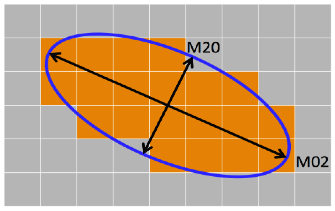
\includegraphics[width=.35\linewidth]{m02&m20.png}
\caption{Schematische Darstellung eines \textit{Clusters}. Die Ellipsenhalbachsen $M_{20}$ und $M_{02}$ definieren eine Ellipse, die alle orange markierten Zellen, die zu einem \textit{Cluster} in einem Kalorimeter mit quadratischen Zellen geh\"ohren, umfasst.
[\cite{thesis:Adrian}]}
\label{fig:$M_{20}$}
\end{figure}
Abbildung \ref{fig:$M_{20}$} zeigt eine schematische Darstellung eines \textit{Clusters}.
Alle orange eingef\"arbten Zellen geh\"oren dabei zu dem \textit{Cluster}.
Die eingezeichnete Ellipse, beziehungsweise ihre Halbachsen $M_{02}$ und $M_{20}$, helfen dabei, das \textit{Cluster} zu parametrisieren.
Die Form eines \textit{Clusters} und damit die Gr\"o{\ss}e von $M_{02}$ und $M_{20}$ unterscheidet sich abh\"angig davon, ob das \textit{Cluster} durch ein Photon entstanden ist oder nicht.
Dadurch kann $M_{02}$ benutzt werden, um \textit{Cluster,} die durch Photonen entstanden sind, zu identifizieren.
Die Teilchen, die zu diesen \textit{Clustern} geh\"oren, werden im Weiteren als Photonenkandidaten bezeichnet.
F\"ur $M_{02}$ gilt:
\begin{align} 
M_{02} = \frac{1}{2}\sum_{i}E_{i}(x_{i}^{2}+y_{i}^{2})+\sqrt{\frac{1}{4}\sum_{i}\left(x_{i}^{2}+y_{i}^{2}\right)^{2}+\left(\sum_{i}E_{i}x_{i}y_{i}\right)}
\end{align}
Wobei $E_{i}$ f\"ur die Energie einer Zelle und $x_{i}$ und $y_{i}$ f\"ur die relative Position einer Zelle zur Startzelle steht.
\newline
Nachdem die Grundlagen zur Theorie und dem Experiment erkl\"art wurden, wird im n\"achsten Abschnitt die Analyse erl\"autert.
Dazu wird zun\"achst die Auswahl der Daten, die in dieser Arbeit benutzt werden, aufgef\"uhrt.